\expandafter\ifx\csname ifdraft\endcsname\relax
   \documentclass[a4j,12pt]{jsreport}
% 数式
\usepackage{amsmath,amsfonts}
\usepackage{bm}

% 画像
\usepackage[dvipdfmx]{graphicx}

% biblatex
\usepackage[style=numeric, sorting=none, maxbibnames=1000]{biblatex}
\addbibresource{graduation_thesis.bib}

%itembox
\usepackage{ascmac}
%breakitemboxのためのpackage
\usepackage{itembkbx}
% \usepackage{tcolorbox} 画像が見えなくなってしまう原因
% \usepackage{framed} 枠

%フォント
\usepackage[ipaex]{pxchfon}

\usepackage[top=35truemm,bottom=30truemm,left=30truemm,right=30truemm]{geometry}
\usepackage{float}
\usepackage{multicol}
\usepackage{multirow}
\usepackage{paralist}
\usepackage{caption}
\usepackage{setspace}
\usepackage{algorithm}
\usepackage{algpseudocode}
\usepackage[dvipdfmx,hidelinks]{hyperref}
\usepackage{pxjahyper}
\usepackage{fancyhdr}
\usepackage{ltablex}
\usepackage{capt-of}
\usepackage{tabularx}
\usepackage{enumitem} % itemizeの行間 これは下になければならない
\usepackage{threeparttable} % 表の脚注


   \setlength{\headheight}{16.5pt}
   \captionsetup{format=hang}
   \begin{document}
   % 上部のヘッダー
\pagestyle{fancy}
\lhead{\rightmark}
\renewcommand{\chaptermark}[1]{\markboth{第\ \thechapter\ 章\ #1}{}}
\fi

\chapter{序論}\label{chap:introduction}
近年, ストリーミングサービスなどメディアコンテンツに関連するサービスが大きな広がりを見せており, 社会におけるメディアコンテンツの流動性が増している. 日々大量のコンテンツが消費され, 次から次へと新しいものが求められるようになった. このようなコンテンツ需要の高まりに応えるストーリー創作の困難は大きい. 多くのコンテンツは, ストーリーを骨格として形成され, その新規性と多様性がコンテンツの魅力と供給に直結するためである. ストーリーの創作には高度な創造性を要し, コンテンツ需要が加速する中, 十分な新しさや多様性をもつ高品質なストーリーを社会の消費に見合う速度で生み出すことに多大な労力が必要になっているのである. このような負担を軽減するため創造性を支援する技術が望まれており, AI技術の応用が期待されている.  

創造性とは, 価値のある新たな発想を生み出す能力のことであり, 価値には, 面白さや美しさ, 有益さといったさまざまな意味が含まれる\cite{boden09}. したがって, ストーリー創作における創造性への支援は, これまでにない面白さをもつ物語への気づきを与えるものであることが望まれる. 

従来のAIがこなせるタスクは単純なものに限られていたため, このような創造性を必要とするタスクに適用することは難しいという議論もあった. しかし現在, より高度で幅広いタスクにも応用可能な Foundation Model\cite{bommasani21}が登場し, AI の適用範囲は創造的活動にまで広がっていると注目されている\cite{frich19}. 特に, GPT-4\cite{OpenAI23} をはじめとした大規模言語モデル(LLM) への期待は大きい. 今日の LLM は, 自然言語処理におけるベンチマークにおいて驚異的な数値を叩き出す\cite{zhao23}. 自然言語を理解しているかのように応答し, 生成される文章は人が書いた文章に匹敵するほどである. 様々な言語タスクに応用可能なLLMの有用さは, 創造性支援にも活用できると考えられ, これまでもストーリークリエーターの創作支援に LLM を用いる試みが行われてきた\cite{ippolito22}.
%自然言語処理分野における様々なタスクで高い性能を発揮するようになっており\cite{ref:Zhao23}, ストーリー創作における創造性支援の可能性を大きく広げている.

しかしながら, その活用方法は未だ確立されていない. LLM から有用な出力を引き出すためにはプロンプトに工夫を施す必要がある\cite{chen23,kojima23,li23}. 例えば, Chain-of-Thought(CoT) プロンプティングと呼ばれるプロンプト技術がある\cite{wei23}. これは図\ref{cot}に示した例のように, 中間的な推論ステップを明示的にプロンプトに盛り込むことで, LLM の推論能力を向上させるものである. このような技術の活用はプロンプトエンジニアリングと呼ばれ, AIに不慣れな人には障壁となると考えられる. したがって, ストーリー創作支援においては, クリエーターのAIに対する理解度に依存しないLLMの効率的な活用を促すその体系の構築が求められている.

\begin{figure}[hbtp]
   \centering
   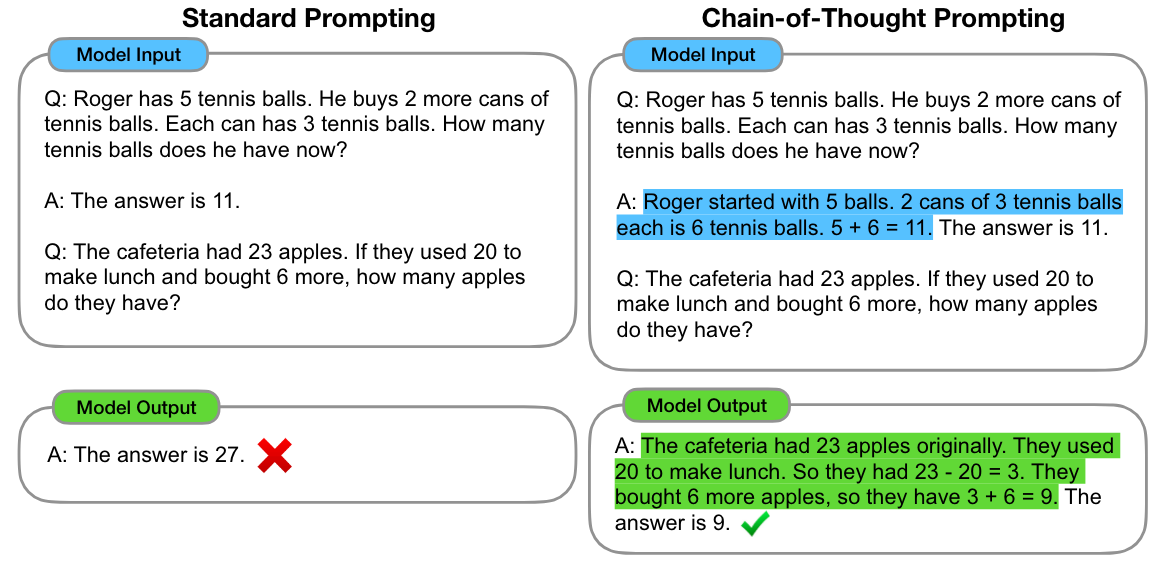
\includegraphics[width=0.8\linewidth]{pict/01/cot.png}
   \caption[Chain-of-Thought プロンプティングの例]{Chain-of-Thought プロンプティングの例 \protect\footnotemark}
   \label{cot}
\end{figure}
\footnotetext{\cite{wei23}より引用}

そこで我々は, 直感的な操作により LLM とのインタラクティブなストーリー共創手法を提供するクリエーターと LLM との仲介システムを web アプリケーションとして開発した. 本システムは, 物語構造分析を活用したLLMの制御を容易な操作により実現するインターフェースと, 繰り返し LLM を作用させることで創造性を高める体系的な創作プロセスを提供する. これらの機能を通じて本システムはストーリークリエーターとLLMとの仲介を担う御用聞きとして機能する.

本研究では, 開発したシステムを「TEZUKA2023プロジェクト\footnotemark \footnotetext{\url{https://tezukaosamu.net/jp/mushi/entry/26751.html} (cited 2024-01-27)}」において手塚治虫の漫画『ブラック・ジャック』\cite{Tezuka77}の新作エピソードの制作に活用してもらい, この取り組みを通じてアンケートの実施と操作ログの取得を行い本システムの有用性について考察した.

なお, 筆者自身の取り組みは以下の通り.
\begin{itemize}
   \item プロンプトの叩き台の提案
   \item プロンプト内における物語構造分析の展開要素の入れ込み方の提案
   \item タイトルおよびあらすじを生成させることの提案
   \item フリーワードによる編集機能の提案
   \item プロット編集セクションにおける一部機能の実装
   \item シナリオ生成セクションにおける一部機能の実装
   \item シナリオ編集セクションにおける一部機能の実装
   \item アンケートの作成
   \item アンケートの分析
   \item 操作ログの分析
\end{itemize}

これらの取り組みについて, プロンプトの叩き台の提案, プロンプト内における物語構造分析の展開要素の入れ込み方の提案については\ref{sec:prompt}節で述べ, タイトルおよびあらすじを生成させることの提案については\ref{self_method}項で, その結果と考察については\ref{self_result}節で, フリーワードによる編集機能の提案については\ref{subsec: freeword}項で, またその結果については\ref{subsec: edit_result}項で, プロット編集セクション等機能の実装については\ref{sec:implementation}節で, アンケートの作成については\ref{quetionnaires}項で, アンケートの分析と操作ログの分析については \ref{quetionnaire_result}節および\ref{log}節で述べる.

本論文の構成は以下の通りである. 第\ref{chap:background}章では, 本研究において開発したシステムが依拠するところの大きい物語構造と大規模言語モデルについて述べ, 第\ref{chap:relatedworks}章では, 関連研究について紹介する. 第\ref{chap:proposedmethod}章では, LLMとのインタラクティブな共創手法を提供するストーリー創作支援システムの提案を行い, 第\ref{chap:experiment}章では, 本システムの有用性を認識するために行われた具体的活用事例について, その詳細と得られた結果および考察について述べる. 最後に第\ref{chap:conclusion}章で結論を述べる.

%そこで我々は, 物語構造を活用し, プロのストーリークリエーターが LLM を用いたストーリー創作を効率的に行うことができる, ユーザーと LLM の仲介を担う御用聞き AI を web アプリとして開発した. このアプリケーションは画面の指示に従う直感的な操作で, 物語構造分析に基づいたプロット生成を実現する. さらに, 生成されたプロットの改善を目的とする, LLM との体系的でインタラクティブな共創手法を提供する. 我々はこのアプリケーションの開発により, LLM を活用したプロのストーリークリエーターの創作支援を探求した.


% \section{本論文の構成}
% 第2章では，ボトムアップ型を取り巻く複雑系という概念を紹介し，階層構造がどのようなものであるかを述べる．
% 第3章では，身体を動的に形成し，身体機能や行動を変化させていく仮想生命体モデルについて紹介する．
% 第4章では，本研究で提案する仮想生命体モデルについて紹介し，構築したシミュレーション環境について述べる．
% 第5章では，シミュレーションの結果とその考察を述べる．
% 第6章では，第5章の内容を元に提案した仮想生命体モデルがどのようであったかについてまとめ，今後の課題について述べる．



\expandafter\ifx\csname ifdraft\endcsname\relax
   \fancyhead[LO]{}
   \printbibliography[title=参考文献]
   \end{document}
   \fancyhead[LO]{\rightmark}
\fi